\documentclass{article}
\usepackage[utf8]{inputenc}
\usepackage{authblk} % To make the adress/email look ok
\usepackage{amsmath} % To use mathematics
\usepackage{tcolorbox} % To use box around text
\usepackage{float}

\title{Labreport - lab 0}
\author{Mohammad Abdulsalam Hajjo}
\affil{Perspectives on Computer Science and Engineering, mohhaj21@student.hh.se}
\date{September 2021}

\begin{document}

\maketitle

\section{Introduction}
This labreport is for us to learn the basics of Matlab. In addition, this labreport is to give us an overview of how to use Overleaf. 

\section{Task 1}
Basically task 1 is just about defining the circle area, adding x and y labels and changing font size. 
\subsection{Code}
\begin{tcolorbox}
\begin{verbatim}
x= linspace(0,10,100);
Area_circle = 2*pi*x.^2;
plot(x,Area_circle,'g')
xlabel('radius/side')
ylabel('Area circle')
ylim([0 700])
ax = gca;
ax.FontSize = 20;
hold on   
\end{verbatim}
\end{tcolorbox} 


\begin{figure}[H]
\centering
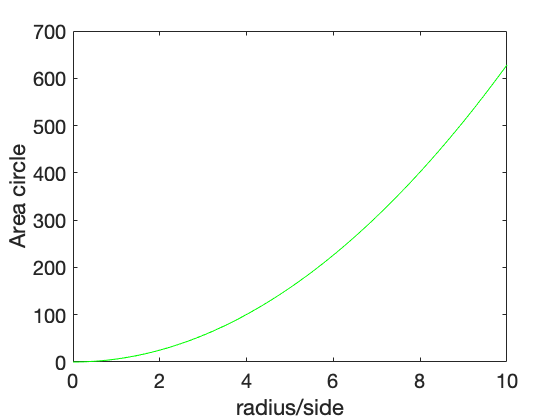
\includegraphics[angle=0,width=8cm]{lab-0 figure1.png}
\caption{Circle area.}
\label{fig:circleAndSquareArea}
\end{figure}


\section{Task 2}
The code for task 2 is a supplement/continuation to task 1. We can say that we paused the code for task 1 to add additional things that are in task 2. For example, we defined the square area and added "legend" and "Grid". In addition we changed the ylabel from "Area circle" to "Area circle/square". 


\subsection{Code}
\begin{tcolorbox}
\begin{verbatim}
Area_square = x.^2;
plot(x,Area_square,'r')
legend({'Circle area','Square area'},'location','northwest')
grid on 
hold off
\end{verbatim}
\end{tcolorbox} 


\section{The whole code}
\begin{tcolorbox}
\begin{verbatim}
x= linspace(0,10,100);
Area_circle = 2*pi*x.^2;
plot(x,Area_circle,'g')
xlabel('radius/side')
ylabel('Area circle/square')
ylim([0 700])
ax = gca;
ax.FontSize = 20;
hold on
Area_square = x.^2;
plot(x,Area_square,'r')
legend({'Circle area','Square area'},'location','northwest')
grid on 
hold off
\end{verbatim}
\end{tcolorbox} 


\begin{figure}[h!]
\centering
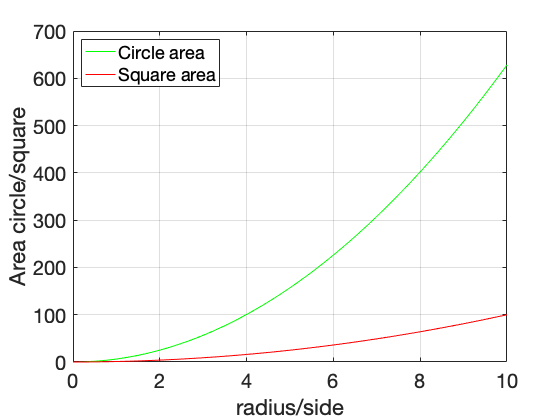
\includegraphics[angle=0,width=8cm]{lab0 _figure2.png}
\caption{Circle and square area plots as functions of side / radius.}
\label{fig:circleAndSquareArea}
\end{figure}


\end{document}